\documentclass[twoside]{article}

% Use the official style file
\usepackage{aistats2026}

% Additional packages (only those you really need)
\usepackage{amsmath, amssymb}
\usepackage{graphicx}
\usepackage{booktabs}
\usepackage{multirow}
\usepackage{algorithm}
\usepackage{algorithmic}
\usepackage{subcaption}
\usepackage{float}

% following three lines:
\usepackage[round]{natbib}
\usepackage{hyperref}
% If you use BibTeX in apalike style, activate the following line:
% \bibliographystyle{apalike}

\begin{document}
% Switch to single-column mode (required for supplementary material)
\onecolumn

% Title
\aistatstitle{Supplementary Materials}

\appendix
\section*{Appendix}
This appendix contains supplementary material that supports the methods and findings in the main paper. It includes:
\begin{itemize}
    \item A. Algorithmic Details: Pseudocode for the two phases of the framework, detector configurations, and hyperparameter settings.
    
    \item B. Statistical Validity: Lemmas justifying the validity of the proposed $p$-values construction and aggregation.

    
    \item C.  List of Generative Models: Comprehensive list of generative models used in evaluation.
    
    \item D.  Full Experimental Results: Detailed baseline comparison table, runtime and memory analysis, robustness evaluations, and qualitative visualization of interpretability.

    \item E. Dataset and Code: Description of released data splits, code and setup for reproducibility.
\end{itemize}

\section{Algorithmic Details}
\label{appendix:pseudocode}
This section provides a detailed algorithmic overview of the phases and the components that constitute our framework.

\subsection{Detectors Configurations}
\label{appendix:detector_config}

\begin{table}[htbp]
\centering
\caption{Configuration of the statistics set used across experiments. Each row specifies the feature extractor and the perturbation strengths \( \lambda \) applied during statistic extraction.}
\begin{tabular}{ll}
\toprule
\textbf{Feature Extractor} & \textbf{Perturbation Strengths \( \lambda \)} \\
\midrule
CLIP ViT-L/14     & 0.05, 0.10 \\
DINOv2 ViT-L/14   & 0.05, 0.10 \\
DINOv3 ViT-S/16   & 0.05, 0.10 \\
DINOv3 ViT-H/16   & 0.05, 0.10 \\
ConvNeXT          & 0.05, 0.10 \\
BEiT ViT-L/16     & 0.05, 0.10 \\
\bottomrule
\end{tabular}
\end{table}

\subsection{Hyperparameter Configurations}
\label{appendix:hyperparams}

The following hyperparameter values were used consistently across all experiments:

\begin{itemize}
    \item Aggregation method: minimum \( p \)-value.
    \item Number of bins for pairwise \(\chi^2\) tests: \( B_{\chi^2} = 15 \).
    \item Number of bins for ECDF estimation: \( B_{\text{ECDF}} = 400 \).
    \item Significance level for KS test of uniformity: \( \alpha_{\text{KS}} = 0.05 \).
    \item Maximum Cramér’s \(V\) threshold for accepting independence in \(\chi^2\) tests: \( V_{\chi^2} = 0.07 \).
\end{itemize}

These values were chosen after exploring a range of configurations during development. Specifically, we evaluated \( B_{\text{ECDF}} \in [200, 1000] \), \( B_{\chi^2} \in [10, 50] \). We also tested thresholds up to \( V_{\chi^2} = 0.1 \) for Cramér’s \(V\) independence criterion and up to \( \alpha_{\text{KS}} = 0.1 \) for the KS uniformity test.

The final configuration was selected based on its empirical stability and the ability to maintain uniformity of aggregated \( p \)-values across different datasets and experimental setups.

\begin{algorithm}[htbp]
\caption{Null Hypothesis Modeling}
\begin{algorithmic}[1]
\STATE \textbf{Input:} Reference dataset $\mathcal{D}_{\text{real}}$
\STATE \textbf{Output:} ECDFs $\{\widehat{F}_{j,k}\}$, Subset $\mathcal{I} \subseteq \mathcal{S}$

\STATE \textit{// Statistic extraction and ECDF modeling (parallelizable)}
\FORALL{detector $(j,k)$} 
    \FORALL{$x_i \in \mathcal{D}_{\text{real}}$} 
        \STATE Compute $s_{j,k}(x_i)$ 
    \ENDFOR
    \STATE Estimate ECDF $\widehat{F}_{j,k}$ from $\{s_{j,k}(x_i)\}$
\ENDFOR

\STATE \textit{// Independence subset selection (pairwise tests are parallelizable)}
\STATE Initialize independence graph $G = (\mathcal{V}, \mathcal{E})$
\FORALL{statistic pairs $(s_i, s_j)$} 
    \STATE Compute Cramér’s $V(s_i, s_j)$ from $\chi^2$ statistic on $p$-values
    \IF{$V(s_i, s_j) \leq V_{\chi^2}$}
        \STATE Add edge $(s_i, s_j)$ to graph $G$
    \ENDIF
\ENDFOR

\STATE Find all cliques in $G$
\STATE Keep cliques passing KS-test with threshold $\alpha_{\text{KS}}$
\STATE Select valid clique maximizing coverage of preferred statistics, breaking ties by size
\end{algorithmic}
\end{algorithm}

\begin{algorithm}[htbp]
\caption{Inference}
\begin{algorithmic}[1]
\STATE \textbf{Input:} Image $x$, ECDFs $\{\widehat{F}_{j,k}\}$, subset $\mathcal{I}$, level $\alpha$
\STATE \textbf{Output:} Decision: \texttt{REAL} or \texttt{FAKE}

\STATE \textit{// Statistic computation and mapping (parallelizable)}
\FORALL{statistic $(j,k) \in \mathcal{I}$}
    \STATE Compute statistic $s_{j,k}(x)$
    \STATE Compute $p$-value $p_{j,k}(x)$ using $\widehat{F}_{j,k}$
\ENDFOR

\STATE Aggregate $\{p_{j,k}(x)\}$ into unified $p$-value (e.g., Stouffer or min-\(p\))
\STATE \textbf{if} unified $p$-value $< \alpha$ \textbf{then return} \texttt{FAKE}
\STATE \textbf{else return} \texttt{REAL}
\end{algorithmic}
\end{algorithm}


\section{Statistical Validity}
\label{appendix:proofs}

This section presents lemmas that justify the statistical validity of our hypothesis testing and $p$-value aggregation procedures. The results establish that the constructed $p$-values are valid under the null hypothesis, assuming independence and i.i.d. real samples.

\subsection*{Lemma 1: Validity of Empirical $p$-Values}

Let \( x \sim \mathbb{P}_{\text{real}} \) and let \( s(x) \) be a scalar statistic. Let \( \widehat{F}_N \) denote the ECDF over \( N \) i.i.d. samples \( x_1, \dots, x_N \sim \mathbb{P}_{\text{real}} \). Define the two-sided empirical $p$-value as
\[
p(x) = 2 \cdot \min\left( \widehat{F}_N(s(x)),\, 1 - \widehat{F}_N(s(x)) \right).
\]
Then under the null hypothesis,
\[
p \sim \mathcal{U}[0,1] \quad \text{as } N \to \infty.
\]


\textit{Note.} This follows directly from the definition of empirical $p$-values. We treat this as a definitional result.

\subsection*{Lemma 2: Stouffer Aggregation Validity}

Let \( p_1, \dots, p_K \sim \mathcal{U}[0,1] \) be independent. Define
\begin{equation}
Z = \frac{1}{\sqrt{K}} \sum_{i=1}^K \Phi^{-1}(p_i)
\end{equation}
\begin{equation}
P_{\text{Stouffer}} = \Phi(Z)
\end{equation}
where \( \Phi \) is the standard normal cumulative distribution function. Then under the null,
\[
P_{\text{Stouffer}} \sim \mathcal{U}[0,1].
\]

\paragraph{Proof.} Since each \( p_i \sim \mathcal{U}[0,1] \), the transformation \( z_i = \Phi^{-1}(p_i) \) yields \( z_i \sim \mathcal{N}(0,1) \). Independence of the \( p_i \)'s implies independence of the \( z_i \)'s. Therefore,
\[
Z = \frac{1}{\sqrt{K}} \sum_{i=1}^K z_i \sim \mathcal{N}(0,1),
\]
and thus \( P_{\text{Stouffer}} = \Phi(Z) \sim \mathcal{U}[0,1] \).
\hfill\(\square\)

\subsection*{Lemma 3: Minimum $p$-Value Aggregation Validity}

Let \( p_1, \dots, p_K \sim \mathcal{U}[0,1] \) independently, and define
\[
P_{\min} = \min_i p_i, \quad F_{P_{\min}}(t) = 1 - (1 - t)^K.
\]
Then under the null,
\[
F_{P_{\min}}(P_{\min}) \sim \mathcal{U}[0,1].
\]

\paragraph{Proof.} For any \( t \in [0,1] \),
\[
\mathbb{P}(P_{\min} \leq t) = 1 - \mathbb{P}(p_1 > t, \dots, p_K > t) = 1 - (1 - t)^K.
\]
Define the transformation
\[
U = F_{P_{\min}}(P_{\min}) = 1 - (1 - P_{\min})^K.
\]
Then for any \( u \in [0,1] \),
\begin{align*}
\mathbb{P}(U \leq u) &= \mathbb{P}\left(P_{\min} \leq 1 - (1 - u)^{1/K}\right) \\
&= F_{P_{\min}}(1 - (1 - u)^{1/K}) = u,
\end{align*}
so \( U \sim \mathcal{U}[0,1] \).
\hfill\(\square\)

\noindent These lemmas ensure that our $p$-value construction and aggregation yield statistically valid outputs under the null hypothesis, assuming independence and i.i.d. sampling from the real distribution.

\section{List of Generative Models}
\label{appendix:generators}

Our evaluation includes synthetic images produced by a diverse range of generative models, drawn from several benchmark datasets: CNNSpot, Universal Fake Detect, Stable-Diffusion-Faces, Synthbuster and GenImage. These datasets collectively span multiple generations of image synthesis techniques and architectural families.

The following models were used in our experiments: ProGAN% \cite{karras2017progressive}
, StyleGAN (WhichFaceIsReal)
, StyleGAN2% \cite{choi2020stargan}
, BigGAN% \cite{brock2018large}
, GauGAN% \cite{park2019semantic}
, CycleGAN% \cite{zhu2017unpaired}
, StarGAN% \cite{choi2018stargan}
, Cascaded Refinement Networks (CRN)% \cite{chen2017photographic}
, Implicit Maximum Likelihood Estimation (IMLE)% \cite{li2019diverse}
, Spatially-Adaptive Normalization (SAN)% \cite{dai2019second}
, DeepFake% \cite{rossler2019learning}
, Stable Diffusion (v1.4, v1.5, v2, XL)%\cite{rombach2022high, podell2023sdxl}
, ADM
, VQDM
, WuKong
, Glide% \cite{nichol2021glide}
, Midjourney v5% \cite{midjourney2023v5}
, and DALL-E 3% \cite{dalle3_openai}
.

% As a source of real reference images, we relied on the real image subsets provided within each benchmark dataset. These include samples drawn from LSUN, %\cite{yu2015lsun},
% MSCOCO, %\cite{lin2014microsoft}, 
% ImageNet %\cite{deng2009imagenet}
%  and LAION%\cite{schuhmann2021laion}.

% This collection spans both academic and commercial generators and provides a rich basis for evaluating generalization across synthesis techniques.

As sources of real images, we relied on benchmark datasets including LSUN, MSCOCO, ImageNet, and LAION. Both our reference and test sets were constructed from these datasets, while ensuring that they consist of disjoint samples. In addition, we incorporated a large number of additional images from MSCOCO that are not part of the predefined benchmark subsets, thereby broadening the diversity and coverage of our real image pool.

\section{Full Experimental Results}
In this section, we present detailed experimental results.

\subsection{Runtime and Memory Usage Analysis}

We evaluated the run-time and memory efficiency of our method across the entire phases of the framework using a representative subset of the MSCOCO dataset and SDXL fake images, 2K images total. All experiments were conducted on a multi-core CPU system and a single NVIDIA A100 80GB GPU, using parallelization with multiple workers.

To assess the scalability of our statistic extraction, we measured its runtime under different GPU worker configurations as the number of selected statistics increases.
\begin{figure}[htbp]
    \centering
    \includegraphics[width=0.45\textwidth]{images/runtime_memory_analysis/statistic_extraction_runtime_by_workers.png}
    \caption{Statistic extraction runtime versus number of statistics under different levels of parallelism. Our method scales efficiently across multiple GPU workers.}
    \label{fig:statistic_extraction_runtime}
\end{figure}
Figure~\ref{fig:statistic_extraction_runtime} confirm that while runtime naturally increases with the number of statistics, our method benefits greatly from parallelism. For instance, with 16 statistics, runtime drops from over 15 minutes with 1 worker to under 8 minutes with 4 workers. At inference time, the per-sample runtime remains low: processing 2000 samples with 4 statistics on a single worker takes only 5.5 minutes, which corresponds to \textbf{0.165 seconds per sample}. This is substantially faster than ManifoldBias and AEROBLADE, which require 2.4 seconds and 5.1 seconds per sample, respectively.

To ensure fair comparison, we limited our evaluation to a single GPU, as baseline methods do not support multi-GPU or multi-process execution. Our implementation, however, is designed for scalability: it distributes computation across multiple workers, reducing CPU-GPU context-switch overhead. Each worker can operate on a separate GPU, compute statistics independently, and return compact ECDFs to the CPU, enabling efficient deployment in both single and multi-GPU environments.

Next, we assess the cost of independence testing and clique selection.
\begin{figure}[htbp]
    \centering
    \includegraphics[width=0.45\textwidth]{images/runtime_memory_analysis/clique_extraction_runtime_analysis.png}
    \caption{Runtime of statistical independence analysis and max-clique selection as the number of statistics increases. Both components scale efficiently.}
    \label{fig:clique_runtime_analysis}
\end{figure}
Figure~\ref{fig:clique_runtime_analysis} demonstrates that both the pairwise \(\chi^2\) matrix computation and the graph-based clique selection remain tractable, even with 32 statistics, requiring under 200ms end-to-end, This supports the practical deployment of our method.

We further evaluate peak GPU memory usage under different configurations and compare it to the baselines.
\begin{figure}[H]
    \centering
    \includegraphics[width=0.45\textwidth]{images/runtime_memory_analysis/peak_gpu_memory_usage.png}
    \caption{Peak GPU memory usage comparison with specified batch size. Our method, achieves high throughput with significantly reduced memory requirements.}
    \label{fig:peak_gpu_memory}
\end{figure}
Figure~\ref{fig:peak_gpu_memory}  shows that our method requires just 7-22GB of GPU memory with 1-4 workers at batch size 128. In contrast, AEROBLADE uses 76GB under the same setup, while ManifoldBias, with 8 internal perturbations, consumes 40GB at batch size 1 and cannot scale to larger batches. Despite using multiple statistics, our method remains memory-efficient and scalable. ECDF storage is also minimal, just 0.25MB for 32 statistics, making the approach practical even on constrained hardware.


Overall, these results demonstrate that our method is not only statistically principled, but also computationally efficient and offering fast inference, strong scalability with GPU workers, and memory usage that is well within practical bounds.

\subsection{Robustness to Image Corruption}

We evaluate robustness to two common real-world image degradations: JPEG compression and Gaussian blur. These corruptions are applied at test time without modifying the original reference distribution, computed ECDFs, or selected statistics \( \mathcal{I} \). All experiments are conducted on the full dataset setup described in Section~C, using the entire test set of both real and fake samples to ensure comprehensive evaluation.

Importantly, metrics are aggregated over all samples, rather than averaged across splits, so that results directly reflect the overall distributional behavior. 

We evaluate robustness to two common degradations:
\begin{itemize}
    \item \textbf{JPEG Compression} (Quality Factor = 0.75) 
    \item \textbf{Standard Gaussian Blur} (3x3 Kernel)
\end{itemize}



\begin{table}[htb]
    \centering
    \small
    \caption{Performance under image corruptions for both ensemble strategies.}
    
    \label{tab:corruption_auc}
    \begin{tabular}{lcccccc}
        \toprule
        \multirow{2}{*}{\textbf{Metric}} & \multicolumn{3}{c}{\textbf{Stouffer}} & \multicolumn{3}{c}{\textbf{MinP}} \\
        \cmidrule(lr){2-4} \cmidrule(lr){5-7}
         & \textbf{Without} & \textbf{JPEG} & \textbf{Blur} & \textbf{Without} & \textbf{JPEG} & \textbf{Blur} \\
        \midrule
        AUC & 0.775 & 0.736 & 0.798 & 0.776 & 0.735 & 0.794 \\
        AP  & 0.798 & 0.750 & 0.818 & 0.786 & 0.734 & 0.807 \\
        \bottomrule
    \end{tabular}
\end{table}


Across both ensemble strategies, JPEG compression leads to a moderate reduction in performance (roughly 5-6\% drop in AUC and AP), but does not induce a significant distributional shift in the $p$-values of real samples, as the null hypothesis remains valid. Gaussian blur introduces minor changes and even improves performance slightly, suggesting that the method is robust to mild smoothing effects regardless of the ensemble variant.

\begin{figure}[H]
\centering

% --- Stouffer figures
\begin{subfigure}[b]{0.31\linewidth}
    \includegraphics[width=\linewidth]{images/robustness/stouffer/before.png}
    \caption{Stouffer: Before corruption}
\end{subfigure}
\hfill
\begin{subfigure}[b]{0.31\linewidth}
    \includegraphics[width=\linewidth]{images/robustness/stouffer/after_jpeg.png}
    \caption{Stouffer: After JPEG}
\end{subfigure}
\hfill
\begin{subfigure}[b]{0.31\linewidth}
    \includegraphics[width=\linewidth]{images/robustness/stouffer/after_blur.png}
    \caption{Stouffer: After blur}
\end{subfigure}

% --- MinP figures
\begin{subfigure}[b]{0.31\linewidth}
    \includegraphics[width=\linewidth]{images/robustness/minp/before.png}
    \caption{Min-$p$: Before corruption}
\end{subfigure}
\hfill
\begin{subfigure}[b]{0.31\linewidth}
    \includegraphics[width=\linewidth]{images/robustness/minp/after_jpeg.png}
    \caption{Min-$p$: After JPEG}
\end{subfigure}
\hfill
\begin{subfigure}[b]{0.31\linewidth}
    \includegraphics[width=\linewidth]{images/robustness/minp/after_blur.png}
    \caption{Min-$p$: After blur}
\end{subfigure}

\caption{
$p$-value distributions for real (blue) and fake (orange) samples under the full dataset setup. 
\textbf{Top row (Stouffer)}: Before corruption (left), after JPEG compression (middle), and after Gaussian blur (right). 
\textbf{Bottom row (Min-$p$)}: Before corruption (left), after JPEG compression (middle), and after Gaussian blur (right). 
Across both ensemble variants, JPEG introduces only a mild shift reducing separability, while Gaussian blur leaves distributions well aligned with the reference, consistent with the observed negligible or positive performance changes.
}
\label{fig:pval_shift_corruptions}
\end{figure}

Overall, these results show that our method remains statistically sound under realistic corruptions: JPEG compression introduces only moderate degradation without violating the null hypothesis, while mild Gaussian blur leaves performance unchanged or slightly improved. The robustness trends are consistent across both Stouffer and Min-$p$ ensembles.

\subsection{Interpretability Qualitative Comparison}
In Figure~\ref{fig:method_interpretability_comparison} we provide a qualitative comparison of interpretability across methods using a shared set of synthetic reference images. Our approach RealStats outputs calibrated $p$-values that quantify image-wise deviation from the reference distribution in an interpretable statistical framework. The resulting scores follow a progression that corresponds to the degree of visual realism, with lower $p$-values indicating a stronger appearance of being fake.

In contrast, the baseline methods, ManifoldBias and Rigid, produce scores whose distances are difficult to interpret. Images with severe visual defects may receive values close to realistic samples, and images from the same semantic domain (e.g., faces) often collapse to similar scores despite substantial corruptions. This lack of calibration limits interpretability, as the scores fail to reflect meaningful distances between samples.
\begin{figure}[H]
\centering
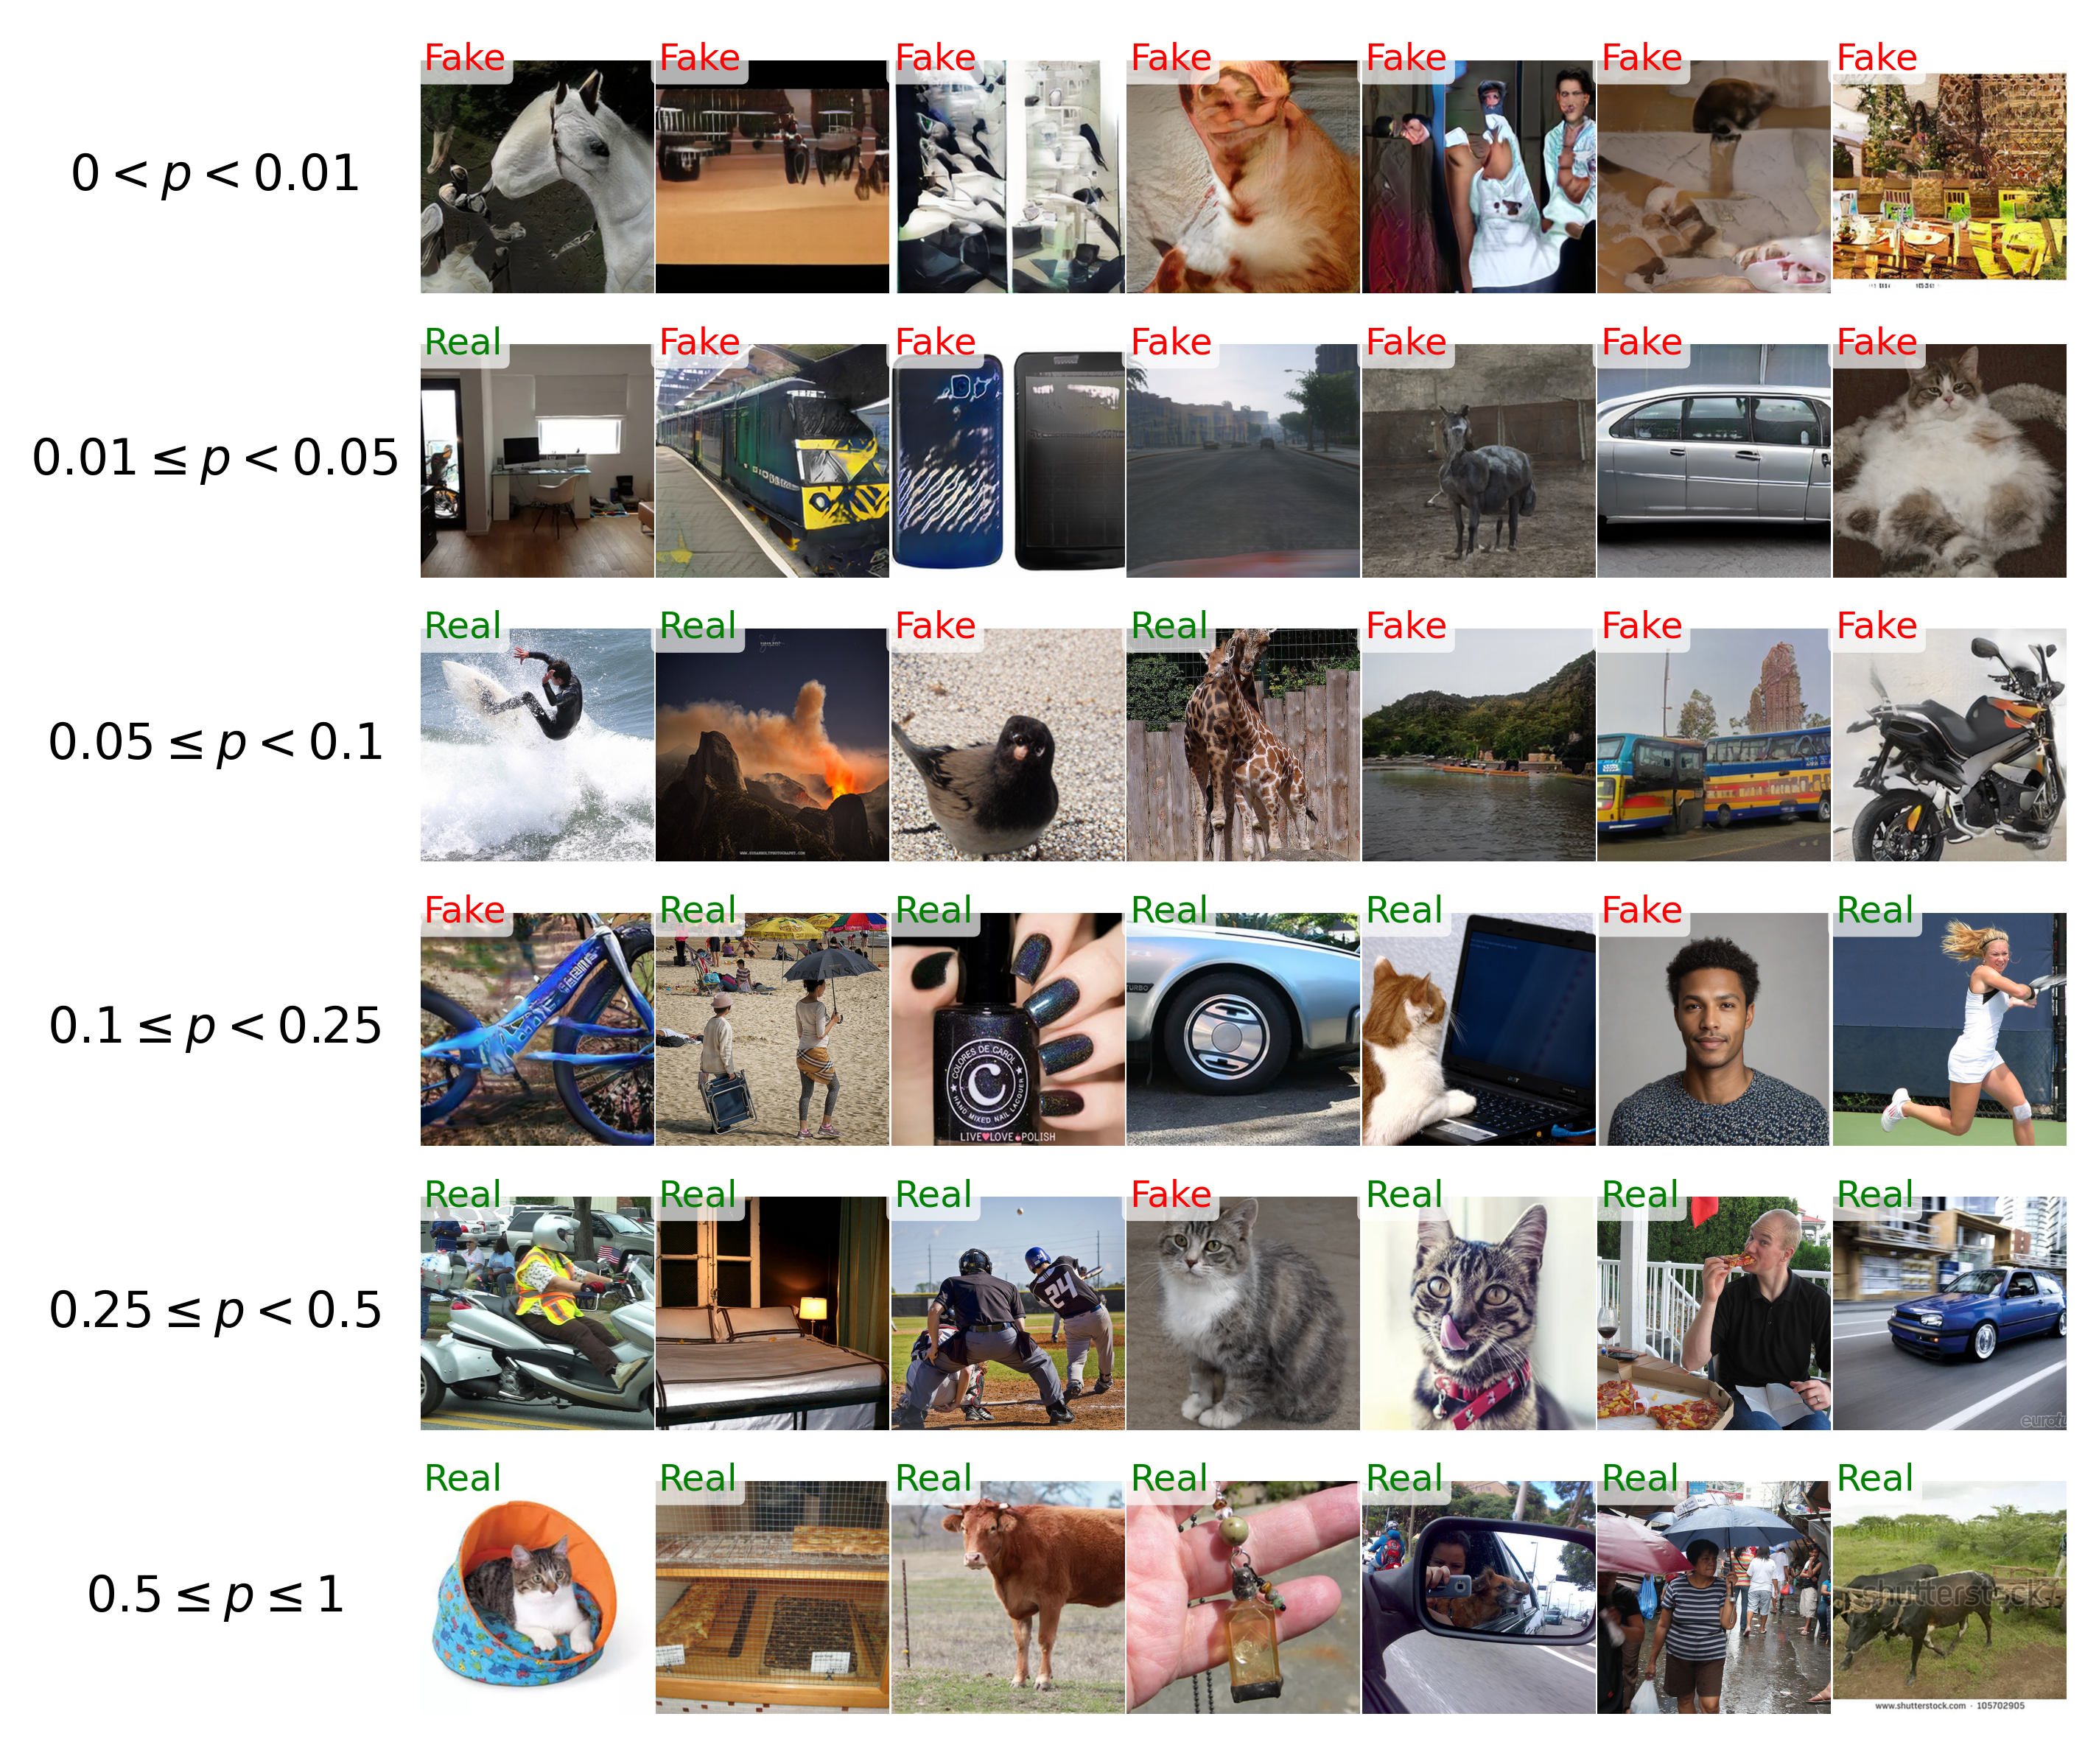
\includegraphics[width=1.0\textwidth]{images/pvalues_distribution/significance_grid.png}
\caption{
\textbf{Qualitative examples of $p$-value trends on test data.}
Images are grouped by $p$-value intervals (low to high). Fake images concentrate at low $p$-values, while a few overlap with real images at higher values, showing statistical similarity to the reference distribution.
}
\label{fig:pvalues_distribution}
\end{figure}
Overall, these results highlight the benefit of using reference-calibrated statistics: while RealStats may not always perfectly separate fake from real, it provides an interpretable scale for reasoning about deviations from the reference distribution.


\begin{figure}[]
    \centering
    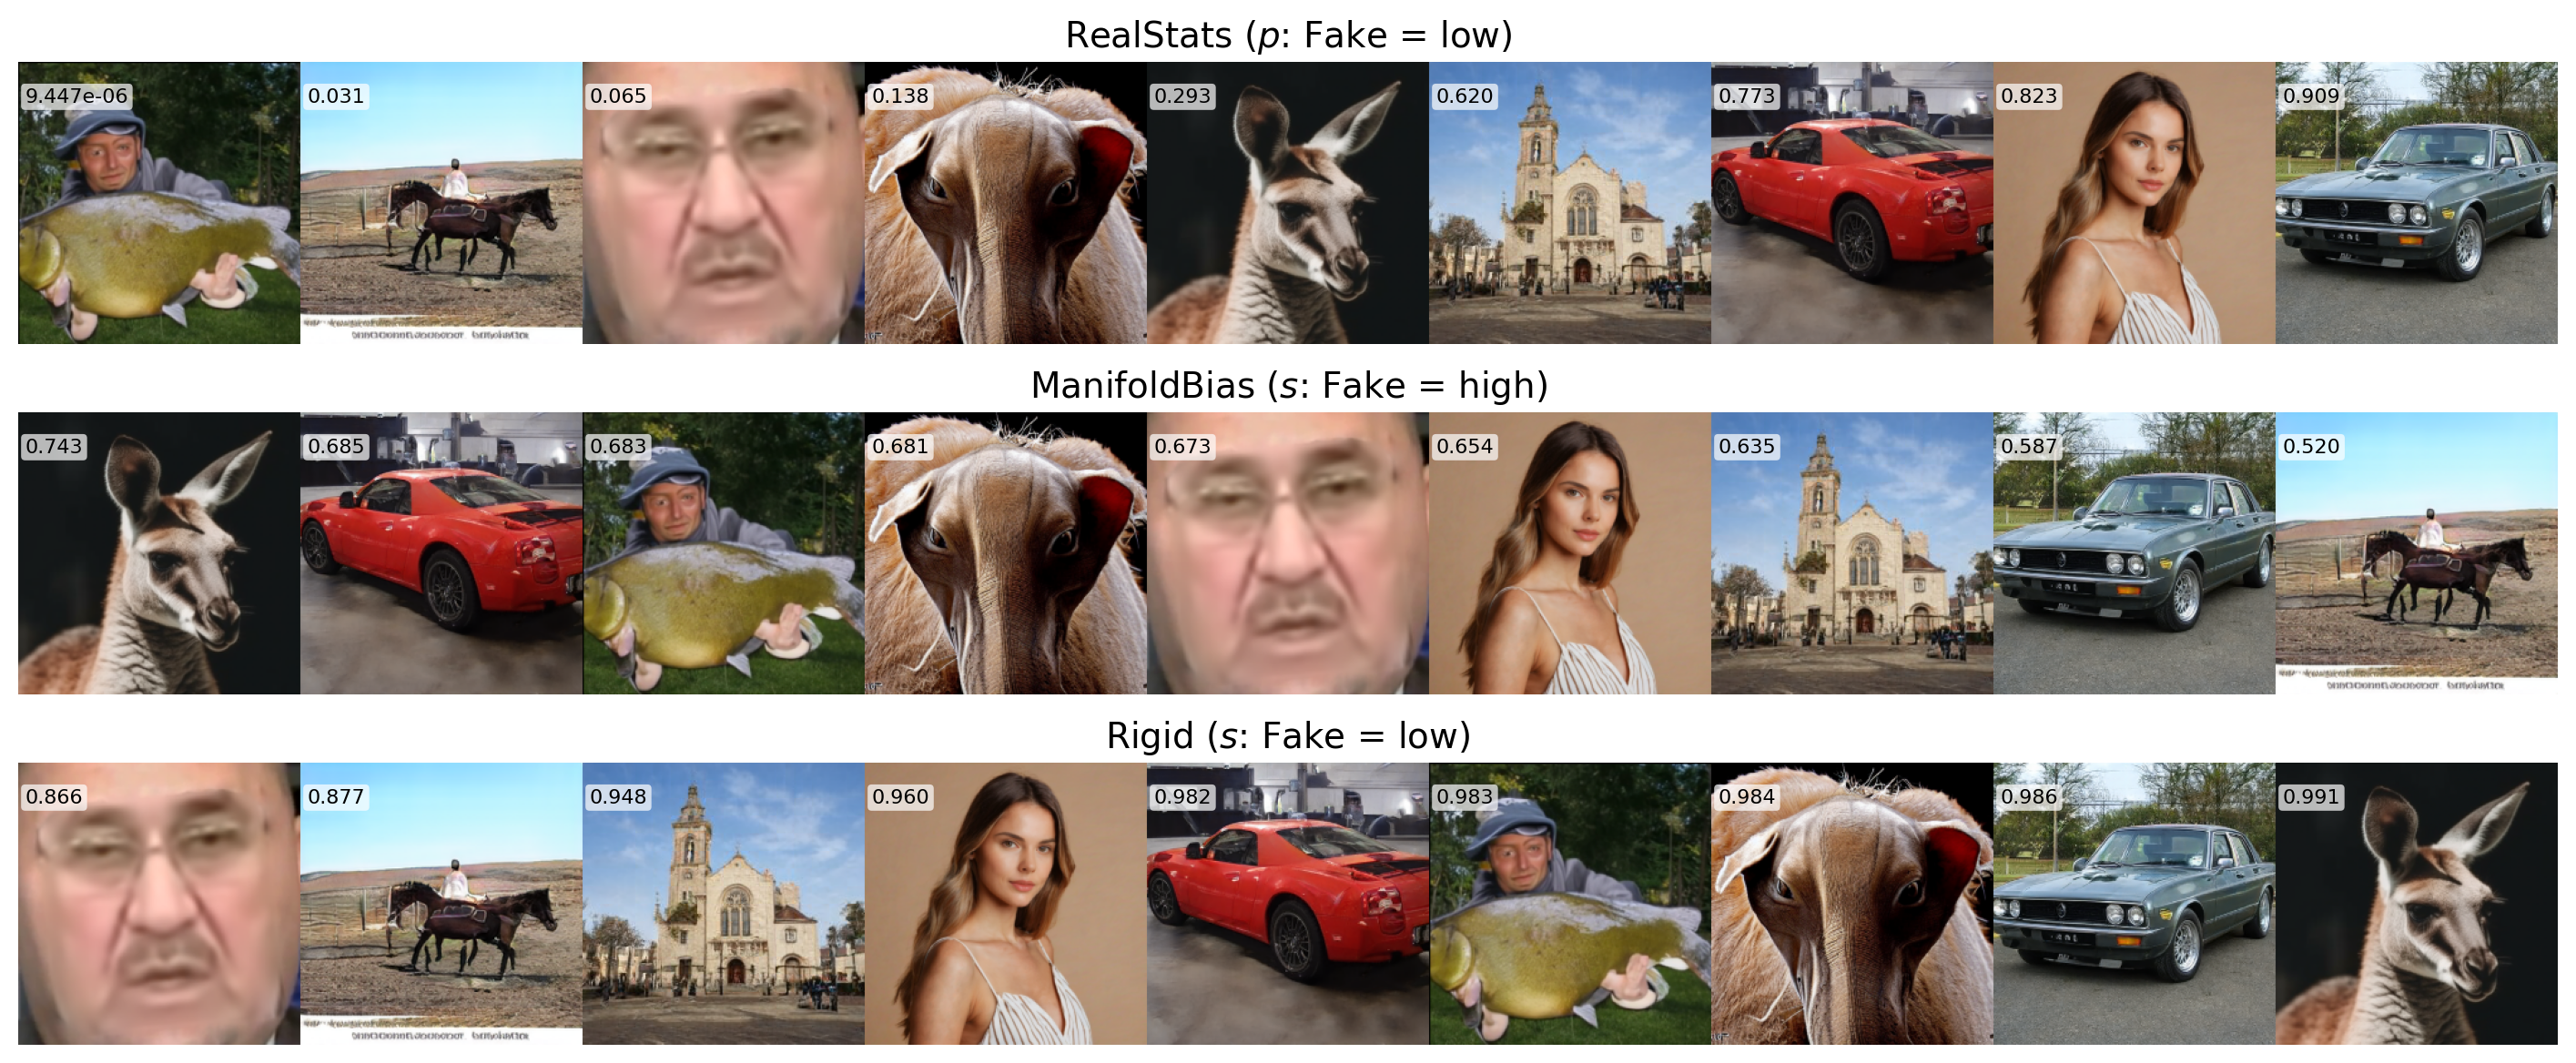
\includegraphics[width=\textwidth]{images/methods_interpretability/method_comparison.pdf}
    \caption{
    \textbf{Qualitative comparison of interpretability across methods.} 
        Each row shows scores assigned by a different method to the same set of fake images. RealStats produces $p$-values that vary consistently with deviation from the reference distribution, while the baselines often cluster visually diverse samples into similar scores.
    }
    \label{fig:method_interpretability_comparison}
\end{figure}

We further illustrate this interpretability by showing $p$-value distributions on our test data (Figure~\ref{fig:pvalues_distribution}). Each row corresponds to a different $p$-value interval, with images annotated by ground-truth labels. Fake images tend to cluster at lower $p$-values, though some appear at higher values, indicating statistical similarity to real images. This visualization highlights how $p$-values provide a calibrated and interpretable measure of sample quality.  

\subsection{Full Table of AUC and AP Values}

Table~\ref{tab:full_auc_ap_bolded} reports the complete per-generator AUC and AP values across all evaluated methods. 
These detailed results complement the averaged scores reported in the paper (Table 1), providing a comprehensive view of method performance for each generator. 
As explained, individual baselines show strong variability across generators while our method maintains competitive and more consistent results overall. 

\begin{table}[!h]
\centering
\caption{AUC and AP scores for each generator across methods.}

\resizebox{\textwidth}{!}{%
\begin{tabular}{lcccccccc}
\toprule
\multirow{2}{*}{Generator} & \multicolumn{4}{c}{AUC} & \multicolumn{4}{c}{AP} \\
 & Ours (Min-$p$) & RIGID & AEROBLADE & ManifoldBias & Ours (Min-$p$) & RIGID & AEROBLADE & ManifoldBias \\
\midrule
ADM & 0.690 & 0.575 & \textbf{0.873} & 0.611 & 0.691 & 0.590 & \textbf{0.845} & 0.564 \\
BigGAN & 0.800 & 0.794 & 0.733 & \textbf{0.909} & 0.773 & 0.798 & 0.747 & \textbf{0.918} \\
CRN & \textbf{0.967} & 0.941 & 0.845 & 0.941 & \textbf{0.930} & 0.924 & 0.836 & 0.915 \\
CycleGAN & 0.785 & 0.787 & 0.706 & \textbf{0.973} & 0.790 & 0.779 & 0.721 & \textbf{0.977} \\
DALLE & 0.552 & 0.588 & \textbf{0.710} & 0.709 & 0.552 & 0.562 & \textbf{0.689} & 0.692 \\
deepfake & 0.926 & \textbf{0.974} & 0.779 & 0.600 & 0.886 & \textbf{0.970} & 0.764 & 0.569 \\
GauGAN & 0.823 & 0.932 & 0.705 & \textbf{0.983} & 0.790 & 0.930 & 0.683 & \textbf{0.983} \\
GLIDE\_100\_27 & 0.920 & \textbf{0.978} & 0.962 & 0.911 & 0.889 & \textbf{0.978} & 0.939 & 0.923 \\
GLIDE\_50\_27 & 0.929 & \textbf{0.982} & 0.964 & 0.920 & 0.905 & \textbf{0.982} & \textbf{0.981} & 0.920 \\
IMLE & \textbf{0.963} & 0.953 & 0.807 & 0.950 & \textbf{0.942} & 0.940 & 0.829 & 0.933 \\
Midjourney & 0.661 & 0.563 & \textbf{0.692} & 0.584 & \textbf{0.661} & 0.531 & 0.705 & 0.564 \\
ProGAN & 0.851 & 0.926 & 0.878 & \textbf{0.957} & 0.845 & 0.923 & 0.902 & \textbf{0.964} \\
SAN & 0.572 & 0.655 & 0.611 & \textbf{0.778} & 0.592 & 0.668 & 0.625 & \textbf{0.780} \\
SDv1.4 & 0.745 & 0.415 & 0.421 & \textbf{0.740} & \textbf{0.720} & 0.423 & 0.444 & 0.646 \\
SDv1.5 & 0.764 & 0.394 & 0.403 & \textbf{0.763} & \textbf{0.750} & 0.414 & 0.391 & 0.674 \\
SDv2 & 0.631 & \textbf{0.820} & 0.450 & 0.587 & 0.623 & \textbf{0.820} & 0.463 & 0.635 \\
SDXL & 0.644 & \textbf{0.853} & 0.612 & 0.534 & 0.605 & \textbf{0.853} & 0.597 & 0.565 \\
StarGAN & 0.876 & \textbf{0.887} & 0.577 & 0.268 & 0.847 & 0.845 & 0.561 & \textbf{0.367} \\
StyleGAN2 & 0.576 & \textbf{0.762} & 0.606 & 0.645 & 0.545 & \textbf{0.747} & 0.584 & 0.685 \\
VQDM & 0.774 & 0.791 & 0.701 & \textbf{0.852} & 0.774 & \textbf{0.809} & 0.718 & 0.848 \\
whichfaceisreal & 0.809 & \textbf{0.946} & 0.823 & 0.744 & 0.769 & \textbf{0.925} & 0.846 & 0.722 \\
Wukong & 0.751 & 0.403 & 0.482 & \textbf{0.751} & \textbf{0.751} & 0.420 & 0.468 & 0.720 \\
\midrule
Average & 0.773 & 0.769 & 0.697 & 0.760 & 0.756 & 0.765 & 0.697 & 0.753 \\
Std & 0.126 & 0.194 & 0.161 & 0.178 & 0.119 & 0.189 & 0.163 & 0.169 \\
\bottomrule
\end{tabular}%
}
\label{tab:full_auc_ap_bolded}
\end{table}

\subsection{Adaptability Scores with ManifoldBias}

The results in Table~\ref{tab:adaptability_full} demonstrate the impact of incorporating adaptability into our ensemble methods. 
By allowing the aggregation strategy to adjust dynamically to different generators, our approach achieves consistently stronger performance, yielding notable improvements in both AUC and AP compared to our base model.
This highlights the importance of adaptability as a key factor for generalization across diverse generative models.

\begin{table}[!h]
\centering
\scriptsize
\caption{Per-generator AUC and AP scores of ensemble methods when integrated with ManifoldBias, with improvements (in \%). Bold indicates positive improvement.}
\begin{tabular}{lcccc}
\toprule
\multirow{2}{*}{Generator} & \multicolumn{2}{c}{AUC} & \multicolumn{2}{c}{AP} \\
 & Min-$p$ & Stouffer & Min-$p$ & Stouffer \\
\midrule
ADM & 0.644 (-6.67\%) & 0.610 & 0.641 (-7.24\%) & 0.594 \\
BigGAN & \textbf{0.869 (+8.62\%)} & 0.865 & \textbf{0.869 (+12.42\%)} & 0.862 \\
CRN & \textbf{0.974 (+0.72\%)} & 0.990 & \textbf{0.956 (+2.80\%)} & 0.986 \\
CycleGAN & \textbf{0.905 (+15.29\%)} & 0.913 & \textbf{0.914 (+15.70\%)} & 0.917 \\
DALLE & \textbf{0.584 (+5.80\%)} & 0.558 & \textbf{0.603 (+9.24\%)} & 0.570 \\
DeepFake & \textbf{0.934 (+0.86\%)} & 0.917 & \textbf{0.903 (+1.92\%)} & 0.886 \\
GauGAN & \textbf{0.949 (+15.31\%)} & 0.936 & \textbf{0.957 (+21.14\%)} & 0.939 \\
Glide\_100\_27 & \textbf{0.941 (+2.28\%)} & 0.951 & \textbf{0.940 (+5.74\%)} & 0.957 \\
Glide\_50\_27 & \textbf{0.948 (+2.05\%)} & 0.962 & \textbf{0.945 (+4.42\%)} & 0.966 \\
IMLE & \textbf{0.973 (+1.04\%)} & 0.993 & \textbf{0.953 (+1.17\%)} & 0.991 \\
Midjourney & 0.518 (-21.63\%) & 0.518 & 0.526 (-20.42\%) & 0.523 \\
ProGAN & \textbf{0.942 (+10.69\%)} & 0.936 & \textbf{0.951 (+12.54\%)} & 0.946 \\
SAN & \textbf{0.670 (+17.13\%)} & 0.668 & \textbf{0.688 (+16.22\%)} & 0.663 \\
SDXL & \textbf{0.646 (+0.31\%)} & 0.645 & \textbf{0.608 (+0.50\%)} & 0.622 \\
SDv2 & \textbf{0.722 (+14.42\%)} & 0.708 & \textbf{0.704 (+13.00\%)} & 0.682 \\
SDv1.4 & 0.689 (-7.52\%) & 0.679 & 0.679 (-5.69\%) & 0.660 \\
SDv1.5 & 0.707 (-7.46\%) & 0.710 & 0.705 (-6.00\%) & 0.706 \\
StarGAN & \textbf{0.887 (+1.26\%)} & 0.864 & \textbf{0.871 (+2.83\%)} & 0.821 \\
StyleGAN2 & \textbf{0.609 (+5.73\%)} & 0.615 & \textbf{0.604 (+10.83\%)} & 0.647 \\
VQDM & \textbf{0.793 (+2.45\%)} & 0.781 & \textbf{0.784 (+1.29\%)} & 0.766 \\
WhichFaceIsReal & \textbf{0.820 (+1.36\%)} & 0.765 & \textbf{0.802 (+4.29\%)} & 0.743 \\
WuKong & 0.707 (-5.86\%) & 0.709 & 0.702 (-6.52\%) & 0.706 \\
\midrule
Average & 0.792 & 0.786 & 0.787 & 0.780 \\
Std & 0.143 & 0.151 & 0.141 & 0.151 \\
\bottomrule
\end{tabular}
\label{tab:adaptability_full}
\end{table}


\section{Datasets and Code}

We release both the \textbf{data splits} used in our experiments and the full \textbf{codebase}. 
The package includes our implementations of \textbf{RIGID statistics} alongside the other statistical measures evaluated in this work, as well as scripts for inference and the complete pipeline. 
We provide the exact \textbf{random seeds} used in all benchmarks and evaluations: \{0, 8, 12, 18, 22, 28, 30, 32, 36, 38\}. 

All resources (code and datasets) are included as a supplementary anonymous ZIP archive and will be made publicly available upon acceptance.

\bibliography{aistats2026}    % loads aistats2026.bib


\end{document}